\documentclass{beamer}
\mode<presentation>
\usepackage{amsmath,amssymb,mathtools}
\usepackage{textcomp}
\usepackage{gensymb}
\usepackage{adjustbox}
\usepackage{subcaption}
\usepackage{enumitem}
\usepackage{multicol}
\usepackage{listings}
\usepackage{url}
\usepackage{graphicx} % <-- needed for images
\def\UrlBreaks{\do\/\do-}

\usetheme{Boadilla}
\usecolortheme{lily}
\setbeamertemplate{footline}{
  \leavevmode%
  \hbox{%
  \begin{beamercolorbox}[wd=\paperwidth,ht=2ex,dp=1ex,right]{author in head/foot}%
    \insertframenumber{} / \inserttotalframenumber\hspace*{2ex}
  \end{beamercolorbox}}%
  \vskip0pt%
}
\setbeamertemplate{navigation symbols}{}

\lstset{
  frame=single,
  breaklines=true,
  columns=fullflexible,
  basicstyle=\ttfamily\tiny   % tiny font so code fits
}

\numberwithin{equation}{section}

% ---- your macros ----
\providecommand{\nCr}[2]{\,^{#1}C_{#2}}
\providecommand{\nPr}[2]{\,^{#1}P_{#2}}
\providecommand{\mbf}{\mathbf}
\providecommand{\pr}[1]{\ensuremath{\Pr\left(#1\right)}}
\providecommand{\qfunc}[1]{\ensuremath{Q\left(#1\right)}}
\providecommand{\sbrak}[1]{\ensuremath{{}\left[#1\right]}}
\providecommand{\lsbrak}[1]{\ensuremath{{}\left[#1\right.}}
\providecommand{\rsbrak}[1]{\ensuremath{\left.#1\right]}}
\providecommand{\brak}[1]{\ensuremath{\left(#1\right)}}
\providecommand{\lbrak}[1]{\ensuremath{\left(#1\right.}}
\providecommand{\rbrak}[1]{\ensuremath{\left.#1\right)}}
\providecommand{\cbrak}[1]{\ensuremath{\left\{#1\right\}}}
\providecommand{\lcbrak}[1]{\ensuremath{\left\{#1\right.}}
\providecommand{\rcbrak}[1]{\ensuremath{\left.#1\right\}}}
\theoremstyle{remark}
\newtheorem{rem}{Remark}
\newcommand{\sgn}{\mathop{\mathrm{sgn}}}
\providecommand{\abs}[1]{\left\vert#1\right\vert}
\providecommand{\res}[1]{\Res\displaylimits_{#1}}
\providecommand{\norm}[1]{\lVert#1\rVert}
\providecommand{\mtx}[1]{\mathbf{#1}}
\providecommand{\mean}[1]{E\left[ #1 \right]}
\providecommand{\fourier}{\overset{\mathcal{F}}{ \rightleftharpoons}}
\providecommand{\system}{\overset{\mathcal{H}}{ \longleftrightarrow}}
\providecommand{\dec}[2]{\ensuremath{\overset{#1}{\underset{#2}{\gtrless}}}}
\newcommand{\myvec}[1]{\ensuremath{\begin{pmatrix}#1\end{pmatrix}}}
\let\vec\mathbf

\title{Matgeo Presentation - Bonus Problem}
\author{ee25btech11063 - Vejith}

\begin{document}


\frame{\titlepage}
\begin{frame}{Question}
Given 3 vectors $\Vec{A}$,$\Vec{B}$,$\Vec{C}$ are coplanar then show det($\Vec{M}$) =0 where\\ $\Vec{M}$=($\Vec{A}$  $\Vec{B}$  $\Vec{C}$)
\end{frame}

\begin{frame}{Solution}
   Equation of plane through 3 coplanar points is 
\begin{align}
    \Vec{n}^T\Vec{x}=0\\
    \implies \Vec{n}^T\Vec{A}= \Vec{n}^T\Vec{B} = \Vec{n}^T\Vec{C}=0\\
    \Vec{M}=(\Vec{A} \hspace{0.5cm} \Vec{B} \hspace{0.5cm} \Vec{C})\\
    \implies \Vec{n}^T\Vec{M}=(\Vec{n}^T\Vec{A} \hspace{0.5cm}  \Vec{n}^T\Vec{B} \hspace{0.5cm} \Vec{n}^T\Vec{C})\\
    \implies \Vec{n}^T\Vec{M}=(0\hspace{0.5cm} 0 \hspace{0.5cm} 0)\\
    \implies \Vec{n}^T\Vec{M}=\Vec{0}
    \end{align}
From (0.6) it means $\Vec{M}$ has a non trivial vector in it$'s$ null space
\begin{align}
    \implies rank(\Vec{M})<3.
\end{align}

For a 3$\times$ 3  square matrix like $\Vec{M}$ if det($\Vec{M}$)$\neq$0 means $\Vec{M}$ is invertible which means $\Vec{M}$ is a full rank matrix\\ 
$\implies$ rank($\Vec{M}$)$=$3.\brak{\text{if det($\Vec{M}$)$\neq$0}}
\end{frame}


\begin{frame}{Solution}
From (0.7)  rank($\Vec{M}$)$<$3 \\
$\implies$ $\Vec{M}$ is not invertible\\
$\implies$ det($\Vec{M}$)$=$0 \\
    \textbf{proof 2}:\\
 3 vectors $\Vec{A}$,$\Vec{B}$,$\Vec{C}$ are coplanar means they are linearly dependent.\\
 let$'$s assume
 \begin{align}
     \Vec{C}=\alpha \Vec{A}+\beta \Vec{B}.\\
     \text{det}(\Vec{M})=\text{det}((\Vec{A} \hspace{0.5cm} \Vec{B} \hspace{0.5cm} \Vec{C})\\
 =\text{det}((\Vec{A} \hspace{0.5cm} \Vec{B} \hspace{0.5cm} \alpha \Vec{A}+\beta \Vec{B})\\
 =\alpha \text{det}((\Vec{A} \hspace{0.5cm} \Vec{B} \hspace{0.5cm} \Vec{A}) + \beta \text{det}((\Vec{A} \hspace{0.5cm} \Vec{B} \hspace{0.5cm} \Vec{B})=0\\
 \implies \text{det}(\Vec{M})=0
 \end{align}
\end{frame}

\begin{frame}{Plot}
    \begin{figure}[H]
    \centering
    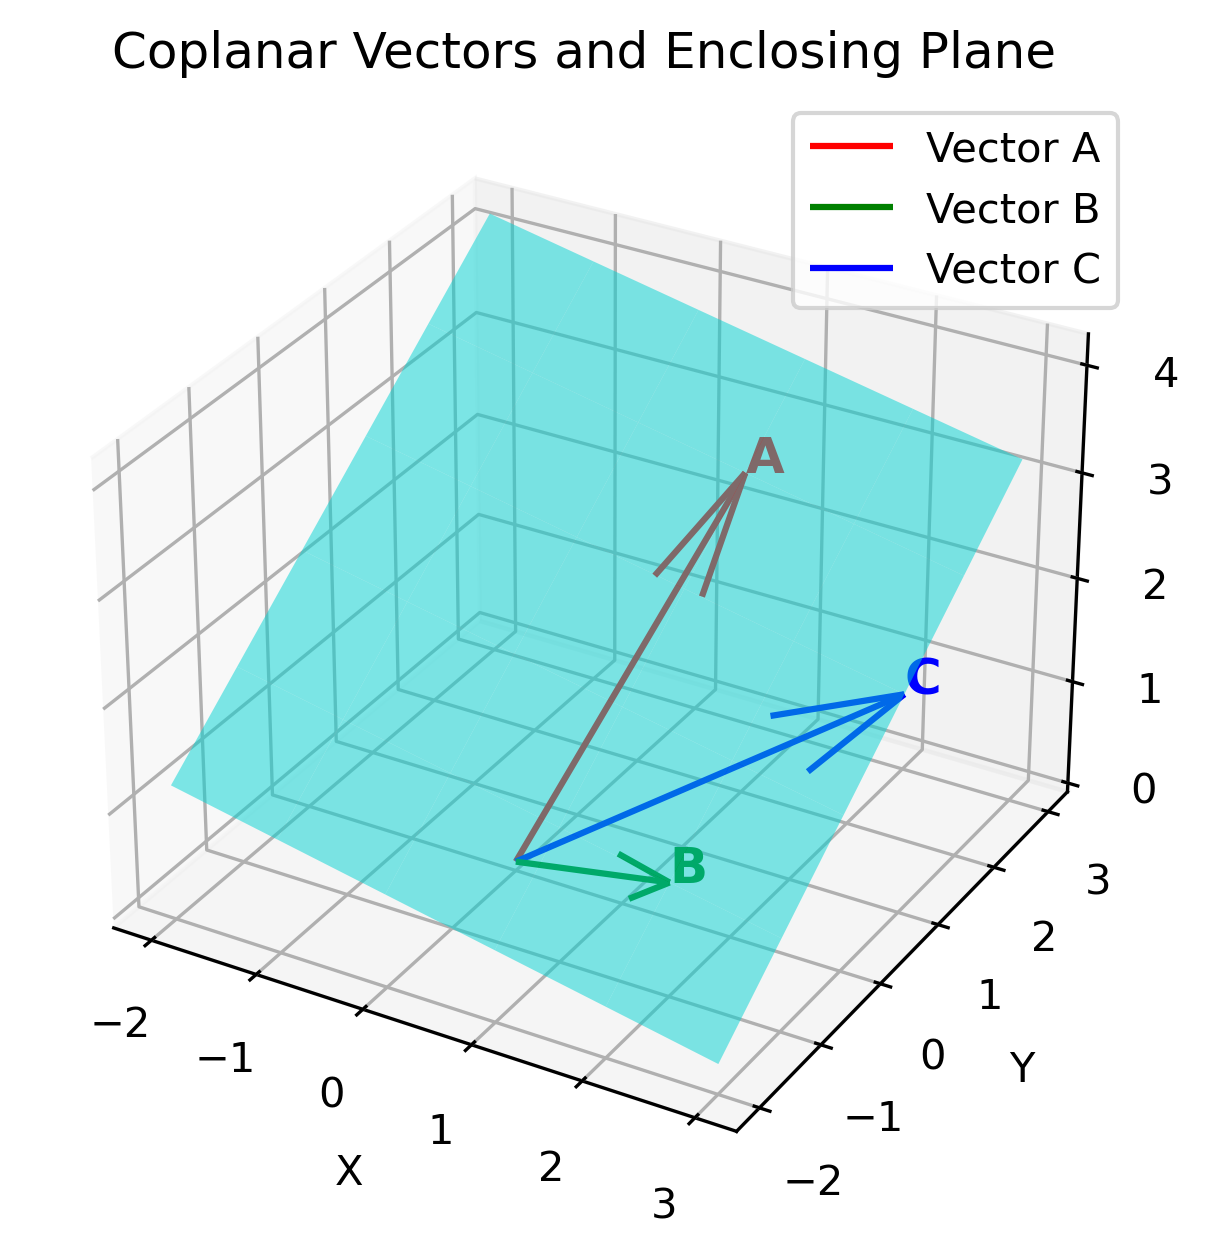
\includegraphics[width=0.60\columnwidth]{figs/01.png}
    \label{fig-1}
\end{figure}
\end{frame}

% --------- CODE APPENDIX ---------
\section*{Appendix: Code}

% C program
\begin{frame}[fragile]{C Code: coplanar.c}
\begin{lstlisting}[language=C]
#include <stdio.h>

#include <stdio.h>

// Function to compute scalar triple product (box product)
float boxProduct(float A[3], float B[3], float C[3]) {
    return A[0] * (B[1]*C[2] - B[2]*C[1])
         - A[1] * (B[0]*C[2] - B[2]*C[0])
         + A[2] * (B[0]*C[1] - B[1]*C[0]);
}

int main() {
    FILE *fp;
    float A[3], B[3], C[3];
    float box;

    // Input 3 vectors
    printf("Enter vector A (x y z): ");
    scanf("%f %f %f", &A[0], &A[1], &A[2]);

    printf("Enter vector B (x y z): ");
    scanf("%f %f %f", &B[0], &B[1], &B[2]);

    printf("Enter vector C (x y z): ");
    scanf("%f %f %f", &C[0], &C[1], &C[2]);

    // Compute box product
    box = boxProduct(A, B, C);

    // Open file coplanar.dat for writing
    fp = fopen("coplanar.dat", "w");
    if (fp == NULL) {
        printf("Error opening file!\n");
        \end{lstlisting}
\end{frame}
\begin{frame}[fragile]{C Code: coplanar.c}
\begin{lstlisting}[language=C]
        return 1;
    }

    fprintf(fp, "Scalar triple product (Box Product) = %.2f\n", box);

    if (box == 0)
        fprintf(fp, "Vectors are coplanar.\n");
    else
        fprintf(fp, "Vectors are NOT coplanar.\n");

    fclose(fp);

    printf("Result written to coplanar.dat\n");

    return 0;
}

\end{lstlisting}
\end{frame}

\begin{frame}[fragile]{Python: plot.py}
\begin{lstlisting}[language=Python]
 import numpy as np
import matplotlib.pyplot as plt
from mpl_toolkits.mplot3d import Axes3D

# ==== Define the vectors ====
A = np.array([1, 2, 3])   # example vector A
B = np.array([2, -1, 1])  # example vector B
C = np.array([3, 1, 2])   # example vector C

# Compute normal to the plane (B-A) × (C-A)
normal = np.cross(B - A, C - A)

# Equation of plane: n·(X - A) = 0  →  n·X = n·A
d = np.dot(normal, A)

# ==== Plotting ====
fig = plt.figure()
ax = fig.add_subplot(111, projection='3d')

# Plot vectors A,B,C from origin (with labels for legend)
ax.quiver(0, 0, 0, A[0], A[1], A[2], color='r', label='Vector A')
ax.quiver(0, 0, 0, B[0], B[1], B[2], color='g', label='Vector B')
ax.quiver(0, 0, 0, C[0], C[1], C[2], color='b', label='Vector C')

# Add labels at arrow tips
ax.text(A[0], A[1], A[2], "A", color='r', fontsize=12, weight='bold')
ax.text(B[0], B[1], B[2], "B", color='g', fontsize=12, weight='bold')
ax.text(C[0], C[1], C[2], "C", color='b', fontsize=12, weight='bold')

# Create grid for the plane
xx, yy = np.meshgrid(range(-2, 4), range(-2, 4))
zz = (d - normal[0]*xx - normal[1]*yy) / normal[2]
\end{lstlisting}
\end{frame} 

\begin{frame}[fragile]{Python: plot.py}
\begin{lstlisting}[language=Python]
# Plot plane
ax.plot_surface(xx, yy, zz, alpha=0.5, color='cyan')

# Labels
ax.set_xlabel('X')
ax.set_ylabel('Y')
ax.set_zlabel('Z')
ax.set_title("Coplanar Vectors and Enclosing Plane")

# Show legend box
ax.legend()

# ==== Save the figure ====
plt.savefig("coplanar_vectors_plane.png", dpi=300, bbox_inches='tight')

plt.show()

\end{lstlisting}
\end{frame} 
\end{document}
